\documentclass[]{book}
\usepackage{lmodern}
\usepackage{amssymb,amsmath}
\usepackage{ifxetex,ifluatex}
\usepackage{fixltx2e} % provides \textsubscript
\ifnum 0\ifxetex 1\fi\ifluatex 1\fi=0 % if pdftex
  \usepackage[T1]{fontenc}
  \usepackage[utf8]{inputenc}
\else % if luatex or xelatex
  \ifxetex
    \usepackage{mathspec}
  \else
    \usepackage{fontspec}
  \fi
  \defaultfontfeatures{Ligatures=TeX,Scale=MatchLowercase}
\fi
% use upquote if available, for straight quotes in verbatim environments
\IfFileExists{upquote.sty}{\usepackage{upquote}}{}
% use microtype if available
\IfFileExists{microtype.sty}{%
\usepackage{microtype}
\UseMicrotypeSet[protrusion]{basicmath} % disable protrusion for tt fonts
}{}
\usepackage[margin=1in]{geometry}
\usepackage{hyperref}
\hypersetup{unicode=true,
            pdftitle={htmlwidgets中文教程},
            pdfauthor={徐静 译},
            pdfborder={0 0 0},
            breaklinks=true}
\urlstyle{same}  % don't use monospace font for urls
\usepackage{natbib}
\bibliographystyle{apalike}
\usepackage{color}
\usepackage{fancyvrb}
\newcommand{\VerbBar}{|}
\newcommand{\VERB}{\Verb[commandchars=\\\{\}]}
\DefineVerbatimEnvironment{Highlighting}{Verbatim}{commandchars=\\\{\}}
% Add ',fontsize=\small' for more characters per line
\usepackage{framed}
\definecolor{shadecolor}{RGB}{248,248,248}
\newenvironment{Shaded}{\begin{snugshade}}{\end{snugshade}}
\newcommand{\KeywordTok}[1]{\textcolor[rgb]{0.13,0.29,0.53}{\textbf{#1}}}
\newcommand{\DataTypeTok}[1]{\textcolor[rgb]{0.13,0.29,0.53}{#1}}
\newcommand{\DecValTok}[1]{\textcolor[rgb]{0.00,0.00,0.81}{#1}}
\newcommand{\BaseNTok}[1]{\textcolor[rgb]{0.00,0.00,0.81}{#1}}
\newcommand{\FloatTok}[1]{\textcolor[rgb]{0.00,0.00,0.81}{#1}}
\newcommand{\ConstantTok}[1]{\textcolor[rgb]{0.00,0.00,0.00}{#1}}
\newcommand{\CharTok}[1]{\textcolor[rgb]{0.31,0.60,0.02}{#1}}
\newcommand{\SpecialCharTok}[1]{\textcolor[rgb]{0.00,0.00,0.00}{#1}}
\newcommand{\StringTok}[1]{\textcolor[rgb]{0.31,0.60,0.02}{#1}}
\newcommand{\VerbatimStringTok}[1]{\textcolor[rgb]{0.31,0.60,0.02}{#1}}
\newcommand{\SpecialStringTok}[1]{\textcolor[rgb]{0.31,0.60,0.02}{#1}}
\newcommand{\ImportTok}[1]{#1}
\newcommand{\CommentTok}[1]{\textcolor[rgb]{0.56,0.35,0.01}{\textit{#1}}}
\newcommand{\DocumentationTok}[1]{\textcolor[rgb]{0.56,0.35,0.01}{\textbf{\textit{#1}}}}
\newcommand{\AnnotationTok}[1]{\textcolor[rgb]{0.56,0.35,0.01}{\textbf{\textit{#1}}}}
\newcommand{\CommentVarTok}[1]{\textcolor[rgb]{0.56,0.35,0.01}{\textbf{\textit{#1}}}}
\newcommand{\OtherTok}[1]{\textcolor[rgb]{0.56,0.35,0.01}{#1}}
\newcommand{\FunctionTok}[1]{\textcolor[rgb]{0.00,0.00,0.00}{#1}}
\newcommand{\VariableTok}[1]{\textcolor[rgb]{0.00,0.00,0.00}{#1}}
\newcommand{\ControlFlowTok}[1]{\textcolor[rgb]{0.13,0.29,0.53}{\textbf{#1}}}
\newcommand{\OperatorTok}[1]{\textcolor[rgb]{0.81,0.36,0.00}{\textbf{#1}}}
\newcommand{\BuiltInTok}[1]{#1}
\newcommand{\ExtensionTok}[1]{#1}
\newcommand{\PreprocessorTok}[1]{\textcolor[rgb]{0.56,0.35,0.01}{\textit{#1}}}
\newcommand{\AttributeTok}[1]{\textcolor[rgb]{0.77,0.63,0.00}{#1}}
\newcommand{\RegionMarkerTok}[1]{#1}
\newcommand{\InformationTok}[1]{\textcolor[rgb]{0.56,0.35,0.01}{\textbf{\textit{#1}}}}
\newcommand{\WarningTok}[1]{\textcolor[rgb]{0.56,0.35,0.01}{\textbf{\textit{#1}}}}
\newcommand{\AlertTok}[1]{\textcolor[rgb]{0.94,0.16,0.16}{#1}}
\newcommand{\ErrorTok}[1]{\textcolor[rgb]{0.64,0.00,0.00}{\textbf{#1}}}
\newcommand{\NormalTok}[1]{#1}
\usepackage{longtable,booktabs}
\usepackage{graphicx,grffile}
\makeatletter
\def\maxwidth{\ifdim\Gin@nat@width>\linewidth\linewidth\else\Gin@nat@width\fi}
\def\maxheight{\ifdim\Gin@nat@height>\textheight\textheight\else\Gin@nat@height\fi}
\makeatother
% Scale images if necessary, so that they will not overflow the page
% margins by default, and it is still possible to overwrite the defaults
% using explicit options in \includegraphics[width, height, ...]{}
\setkeys{Gin}{width=\maxwidth,height=\maxheight,keepaspectratio}
\IfFileExists{parskip.sty}{%
\usepackage{parskip}
}{% else
\setlength{\parindent}{0pt}
\setlength{\parskip}{6pt plus 2pt minus 1pt}
}
\setlength{\emergencystretch}{3em}  % prevent overfull lines
\providecommand{\tightlist}{%
  \setlength{\itemsep}{0pt}\setlength{\parskip}{0pt}}
\setcounter{secnumdepth}{5}
% Redefines (sub)paragraphs to behave more like sections
\ifx\paragraph\undefined\else
\let\oldparagraph\paragraph
\renewcommand{\paragraph}[1]{\oldparagraph{#1}\mbox{}}
\fi
\ifx\subparagraph\undefined\else
\let\oldsubparagraph\subparagraph
\renewcommand{\subparagraph}[1]{\oldsubparagraph{#1}\mbox{}}
\fi

%%% Use protect on footnotes to avoid problems with footnotes in titles
\let\rmarkdownfootnote\footnote%
\def\footnote{\protect\rmarkdownfootnote}

%%% Change title format to be more compact
\usepackage{titling}

% Create subtitle command for use in maketitle
\newcommand{\subtitle}[1]{
  \posttitle{
    \begin{center}\large#1\end{center}
    }
}

\setlength{\droptitle}{-2em}

  \title{htmlwidgets中文教程}
    \pretitle{\vspace{\droptitle}\centering\huge}
  \posttitle{\par}
    \author{徐静 译}
    \preauthor{\centering\large\emph}
  \postauthor{\par}
      \predate{\centering\large\emph}
  \postdate{\par}
    \date{2018-07-05}

\usepackage{booktabs}
\usepackage{xeCJK}

\setCJKmainfont{宋体}

\setmainfont{Georgia}

\setromanfont{Georgia}

\setmonofont{Courier New}

\usepackage{amsthm}
\newtheorem{theorem}{Theorem}[chapter]
\newtheorem{lemma}{Lemma}[chapter]
\theoremstyle{definition}
\newtheorem{definition}{Definition}[chapter]
\newtheorem{corollary}{Corollary}[chapter]
\newtheorem{proposition}{Proposition}[chapter]
\theoremstyle{definition}
\newtheorem{example}{Example}[chapter]
\theoremstyle{definition}
\newtheorem{exercise}{Exercise}[chapter]
\theoremstyle{remark}
\newtheorem*{remark}{Remark}
\newtheorem*{solution}{Solution}
\begin{document}
\maketitle

{
\setcounter{tocdepth}{1}
\tableofcontents
}
\chapter*{声明}
\addcontentsline{toc}{chapter}{声明}

\href{https://CRAN.R-project.org/package=htmlwidgets}{htmlwidgets}是R语言中非常有划时代意义的包,因为有了htmlwidgets使得R语言在交互可视化和基于JavaScript的编程有了实质性的进步。htmlwidgets目前没有中文说明文档和教程,该文档是对官方文档的详细翻译,译者水平有限,读者可以在\url{https://github.com/DataXujing/htmlwidgets_CN/issues}中留言指正。

\begin{center}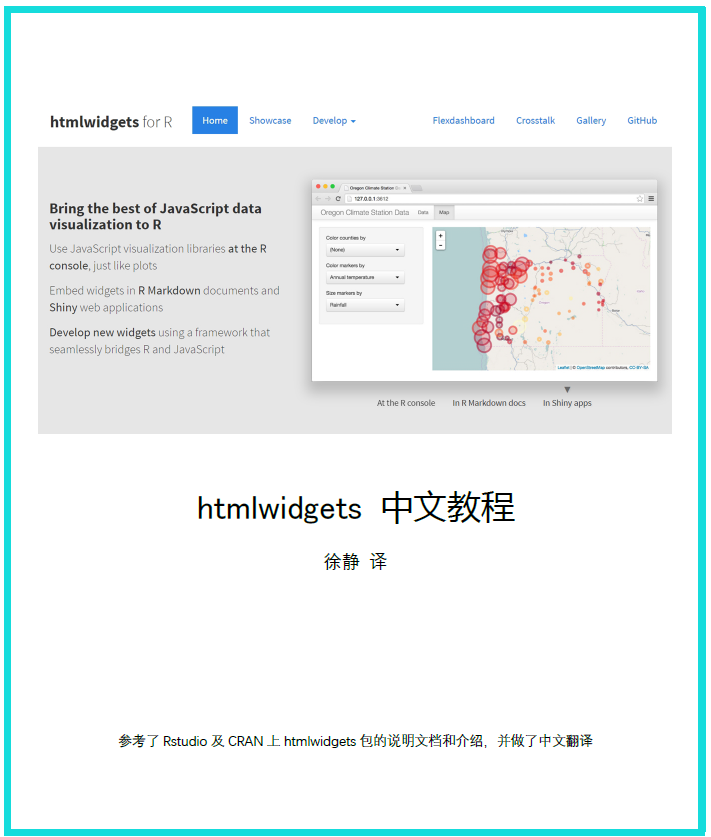
\includegraphics[width=9.88in,height=0.7\textheight]{pic/cover} \end{center}

\chapter*{序言}
\addcontentsline{toc}{chapter}{序言}

htmlwidgets,一个用来创建HTML控件的包,可以运行在R命令行, R Markdown,
Shiny。

\begin{verbatim}
Type Package
Title HTML Widgets for R
Version 1.2
Description A framework for creating HTML widgets that render in various
contexts including the R console, 'R Markdown' documents, and 'Shiny'
web applications.
License MIT + file LICENSE
VignetteBuilder knitr
Imports grDevices, htmltools (>= 0.3), jsonlite (>= 0.9.16), yaml
Suggests knitr (>= 1.8)
Enhances shiny (>= 1.0.5)
URL https://github.com/ramnathv/htmlwidgets
BugReports https://github.com/ramnathv/htmlwidgets/issues
RoxygenNote 6.0.1
NeedsCompilation no
Author Ramnath Vaidyanathan [aut, cph],Yihui Xie [aut],JJ Allaire [aut, cre],Joe Cheng [aut],
Kenton Russell [aut, cph],RStudio [cph]
Maintainer JJ Allaire <jj@rstudio.com>
Repository CRAN
Date/Publication 2018-04-19 12:43:03 UTC
\end{verbatim}

目前针对于htmlwidgets并没有详细的中文教程,译者会持续更新翻译htmlwidgets,并推出更多基于htmlwidgets的R包。

徐静

联信商务咨询有限公司

2017-06-02

\chapter*{关于译者}
\addcontentsline{toc}{chapter}{关于译者}

\textbf{徐静:}

硕士研究生,
目前的研究兴趣主要包括:数理统计,统计机器学习,深度学习,网络爬虫,前端可视化,R语言和Python语言的超级粉丝,多个R包和Python模块的作者,现在正逐步向Java迁移。

Graduate students,the current research interests include: mathematical
statistics, statistical machine learning, deep learning, web crawler,
front-end visualization. He is a super fan of R and Python, and the
author of several R packages and Python modules, and now gradually
migrating to Java.

\chapter{简介}\label{htmlwidgets-intro}

\section{概况}

\href{https://cran.r-project.org/web/packages/htmlwidgets/index.html}{htmlwidgets}包提供了一个R语言链接Javascript库的框架,HTML控件能够:

\begin{itemize}
\item
  在R命令中做分析比如方便的R作图
\item
  和R Markdown结合在一起
\item
  和shiny结合在一起
\item
  保存为独立的网页,通过电子邮件,Dropbox等ad-oc共享。
\end{itemize}

通过遵循一小部分易于遵循的约定,可以创建非常小的代码和HTML控件,所有控件包含如下部分:

\begin{enumerate}
\def\labelenumi{\arabic{enumi}.}
\item
  \emph{Dependencies}: 这些是控件用到的需要声明的Javascript和CSS
\item
  \emph{R binding}:
  这是终端用户将调用的功能,以向控件提供输入数据,并制定控件应该如何呈现各种选项,这包括在shiny应用程序中使用控件所需要的一些简短的样板功能。
\item
  \emph{javaScript binding}:
  这是JavaScript代码,把所有的东西粘在一起。将R绑定中收集的数据和选项传递给底层的JavaScript库
\end{enumerate}

已经有非常多的包基于htmlwidgets去完成,包括:

\begin{itemize}
\item
  leaflet -- 交互的地图绘制包
\item
  dygraphs -- 交互时间序列绘图包
\item
  networkD3 -- 基于D3.js的交互网络图可视化
\item
  sparkline -- 小型的内联图
\item
  DT -- 表格可视化
\item
  rthreejs -- 交互3D图
\end{itemize}

包的作者包括:Ramnath Vaidyanathan, Joe Cheng, JJ Allaire, Yihui Xie,
and Kenton Russell等。

HTML控件一般会寄存在一个R包中,并且应该包含他们的依赖关系的所有源代码,例如这里译者写的以个基于htmlwidgets的R包:\href{https://github.com/DataXujing/XuJIngd3plus}{XuJIngd3plus}。这是为了确保依赖的控件的完全可重复的(既不需要联网,也不需要运行服务器),说白了在你R包中,应该包含所有的源码包括你底层调用的JavaScript包或CSS。

\section{简单的开始}

如果你懂R语言和一点JavaScript,创建自己的小控件非常简单,最先要做的就是要安装htmlwidgets,在CRAN上:

\begin{Shaded}
\begin{Highlighting}[]
\KeywordTok{install.packages}\NormalTok{(}\StringTok{'htmlwidgets'}\NormalTok{)}
\end{Highlighting}
\end{Shaded}

你也可以在GitHub上安装开发版本:

\begin{Shaded}
\begin{Highlighting}[]
\NormalTok{devtools}\OperatorTok{::}\KeywordTok{install_github}\NormalTok{(}\StringTok{'ramnathv/htmlwidgets'}\NormalTok{)}
\end{Highlighting}
\end{Shaded}

通过包中自带的说明文档,让你快速的熟悉htmlwidgets并进入开发者状态,包括:

\begin{itemize}
\item
  Introduction to HTML Widgets
\item
  HTML Widget Sizing
\item
  HTML Widgets: Advanced Topics
\end{itemize}

我们会持续把他们翻译成中文,让中国人看起来更爽。

\section{例子(sigma.js)}\label{sigma.js}

首先,我们将通过创建一个控件来封装\href{http://sigmajs.org/}{sigma.js}图形可视化库。当我们完成后,我们可以用来显示\href{https://gephi.org/gexf/format/}{GEXF}(Graph
Exchange XML Format)数据文件的交互可视化,例如:

\begin{Shaded}
\begin{Highlighting}[]
\KeywordTok{library}\NormalTok{(sigma)}
\NormalTok{data <-}\StringTok{ }\KeywordTok{system.file}\NormalTok{(}\StringTok{"examples/ediaspora.gexf.xml"}\NormalTok{, }\DataTypeTok{package =} \StringTok{"sigma"}\NormalTok{)}
\KeywordTok{sigma}\NormalTok{(data)}
\end{Highlighting}
\end{Shaded}

\begin{center}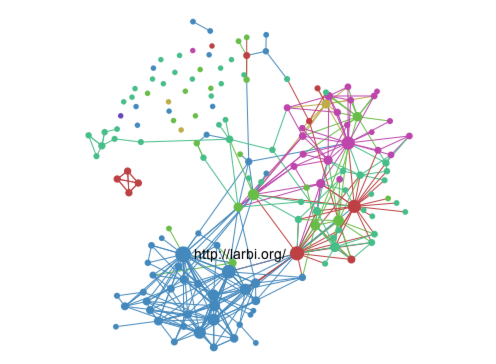
\includegraphics[width=6.89in]{pic/ch1_1} \end{center}

注意上面的输出仅仅是一个静态图像,你可以按照下文的Demo做一个交互的版本。

创建这种绑定所需的代码非常少。下面我们将一步一步地介绍所有的控件。然后,我们将描述如何创建自己的控件(包括为所有核心组件自动生成基本的脚手架)。

\subsection{文件布局}

假设我们的控件被命名为\textbf{sigma},并且位于同名的R包中。我们的JavaScript绑定源代码文件名为sigma.js。由于我们的控件将读取GEXF数据文件,我们还需要包括基础sigma.min.js库以及GEXF插件,下面是我们将添加到包中的文件:

\begin{verbatim}
R/
| sigma.R

inst/
|-- htmlwidgets/
|   |-- sigma.js
|   |-- sigma.yaml
|   |-- lib/
|   |   |-- sigma-1.0.3/
|   |   |   |-- sigma.min.js
|   |   |   |-- plugins/
|   |   |   |   |-- sigma.parsers.gexf.min.js
\end{verbatim}

请注意,JavaScript,YAML和其他依赖项都包含在inst/htmlwidgets目录中(随后将被安装到一个名为htmlwidgets的包的子目录中)。

\subsection{依赖关系}

依赖项是控件使用的JavaScript和CSS资源。依赖项包含在inst/htmlwidgets/lib目录中。依赖关系是使用YAML配置文件指定的,该文件使用控件的名称作为其基本文件名。以下是我们的sigma.yaml文件的样子

\begin{verbatim}
dependencies:
  - name: sigma
    version: 1.0.3
    src: htmlwidgets/lib/sigma-1.0.3
    script: 
      - sigma.min.js
      - plugins/sigma.parsers.gexf.min.js
\end{verbatim}

依赖关系src详述了引用目录,包含库和指定的JavaScript代码文件。如果包含多个JS脚本,每一个占每一行,并且以`-开头。同时你可以天剑stylesheet条目,还有元条目或头条目,多依赖关系可以在一个YAML文件中声明,更多的请参考htmlDependency函数,该函数在\href{https://cran.r-project.org/web/packages/htmltools/index.html}{htmltools}包中

\subsection{R绑定(R binding)}\label{rr-binding}

我们需要为用户提供一个调用我们的控件的R函数。通常,该函数将接受输入数据以及控制控件的显示的各种选项。下面是sigma的R函数:

\begin{Shaded}
\begin{Highlighting}[]
\CommentTok{#' @import htmlwidgets}
\CommentTok{#' @export}
\NormalTok{sigma <-}\StringTok{ }\ControlFlowTok{function}\NormalTok{(gexf, }\DataTypeTok{drawEdges =} \OtherTok{TRUE}\NormalTok{, }\DataTypeTok{drawNodes =} \OtherTok{TRUE}\NormalTok{,}
                  \DataTypeTok{width =} \OtherTok{NULL}\NormalTok{, }\DataTypeTok{height =} \OtherTok{NULL}\NormalTok{) \{}
  
  \CommentTok{# read the gexf file}
\NormalTok{  data <-}\StringTok{ }\KeywordTok{paste}\NormalTok{(}\KeywordTok{readLines}\NormalTok{(gexf), }\DataTypeTok{collapse=}\StringTok{"}\CharTok{\textbackslash{}n}\StringTok{"}\NormalTok{)}
  
  \CommentTok{# create a list that contains the settings}
\NormalTok{  settings <-}\StringTok{ }\KeywordTok{list}\NormalTok{(}
    \DataTypeTok{drawEdges =}\NormalTok{ drawEdges,}
    \DataTypeTok{drawNodes =}\NormalTok{ drawNodes}
\NormalTok{  )}
  
  \CommentTok{# pass the data and settings using 'x'}
\NormalTok{  x <-}\StringTok{ }\KeywordTok{list}\NormalTok{(}
    \DataTypeTok{data =}\NormalTok{ data,}
    \DataTypeTok{settings =}\NormalTok{ settings}
\NormalTok{  )}
  
  \CommentTok{# create the widget}
\NormalTok{  htmlwidgets}\OperatorTok{::}\KeywordTok{createWidget}\NormalTok{(}\StringTok{"sigma"}\NormalTok{, x, }\DataTypeTok{width =}\NormalTok{ width, }\DataTypeTok{height =}\NormalTok{ height)}
\NormalTok{\}}
\end{Highlighting}
\end{Shaded}

函数包含两类输入:GEXF数据文件和一些附加的设置参数用来控制如何显示图片。这些输入都集中在一个叫做x的列表中,然后灌入到htmlwidgets::createWidget函数。这个x变量随后将被用于sigma的JavaScript绑定(下面将对此进行描述),指定的任何宽度或高度参数也会被转发到widget(默认情况下,控件自动调整大小,因此通常不需要显式的宽度或高度)。

我们也希望sigma控件能够在shiny应用中使用,因此我们添加了下面的公式化的shiny
output和render函数(对于所有的控件来说,它总是相同的)

\begin{Shaded}
\begin{Highlighting}[]
\CommentTok{#' @export}
\NormalTok{sigmaOutput <-}\StringTok{ }\ControlFlowTok{function}\NormalTok{(outputId, }\DataTypeTok{width =} \StringTok{"100%"}\NormalTok{, }\DataTypeTok{height =} \StringTok{"400px"}\NormalTok{) \{}
\NormalTok{  htmlwidgets}\OperatorTok{::}\KeywordTok{shinyWidgetOutput}\NormalTok{(outputId, }\StringTok{"sigma"}\NormalTok{, width, height, }\DataTypeTok{package =} \StringTok{"sigma"}\NormalTok{)}
\NormalTok{\}}
\CommentTok{#' @export}
\CommentTok{#https://blog.csdn.net/songzhilian22/article/details/49487467}
\NormalTok{renderSigma <-}\StringTok{ }\ControlFlowTok{function}\NormalTok{(expr, }\DataTypeTok{env =} \KeywordTok{parent.frame}\NormalTok{(), }\DataTypeTok{quoted =} \OtherTok{FALSE}\NormalTok{) \{}
  \ControlFlowTok{if}\NormalTok{ (}\OperatorTok{!}\NormalTok{quoted) \{ expr <-}\StringTok{ }\KeywordTok{substitute}\NormalTok{(expr) \} }\CommentTok{# force quoted}
\NormalTok{  htmlwidgets}\OperatorTok{::}\KeywordTok{shinyRenderWidget}\NormalTok{(expr, sigmaOutput, env, }\DataTypeTok{quoted =} \OtherTok{TRUE}\NormalTok{)}
\NormalTok{\}}
\end{Highlighting}
\end{Shaded}

\subsection{JavaScript绑定(JavaScript
binding)}\label{javascriptjavascript-binding}

注意:在htmlwidgets0.5.2和更早的版本中使用了一个更老、更不直观的JavaScript绑定API,并在htmlwidgets的更新版本中继续支持。有关遗留绑定API的详细信息,请参见此归档版本。新的控件件被鼓励使用下面描述的更新的API。谜题中的第三个部分是激活控件所需的JavaScript。按照惯例,我们将在文件inst/htmlwidgets/sigma.js中定义JavaScript绑定。下面是绑定的完整源代码:

\begin{verbatim}
HTMLWidgets.widget({

  name: "sigma",
  
  type: "output",
  
  factory: function(el, width, height) {
  
    // create our sigma object and bind it to the element
    var sig = new sigma(el.id);
    
    return {
      renderValue: function(x) {
          
        // parse gexf data
        var parser = new DOMParser();
        var data = parser.parseFromString(x.data, "application/xml");
        
        // apply settings
        for (var name in x.settings)
          sig.settings(name, x.settings[name]);
        
        // update the sigma object
        sigma.parsers.gexf(
          data,          // parsed gexf data
          sig,           // sigma object
          function() {
            // need to call refresh to reflect new settings and data
            sig.refresh();
          }
        );
      },
      
      resize: function(width, height) {
        
        // forward resize on to sigma renderers
        for (var name in sig.renderers)
          sig.renderers[name].resize(width, height);  
      },
      
      // Make the sigma object available as a property on the widget
      // instance we're returning from factory(). This is generally a
      // good idea for extensibility--it helps users of this widget
      // interact directly with sigma, if needed.
      s: sig
    };
  }
});
\end{verbatim}

我们为控件提供了名称和类型,再加上一个工厂函数,它采用el(将承载这控件的HTML元素)、宽度和高度(HTML元素的宽度和高度,以像素为单位),您总是可以使用OffStStand宽度和OffSETHEE来实现这一点。

工厂函数要准备启动接收HTML元素的值。在这个案例,我们创建一个新的sigma元素和把它的DOM元素的ID,承载页面的控件。

我们稍后需要访问sigma对象(以更新它的数据和设置),因此我们将其保存为变量sig。请注意,直接在工厂函数内部声明的变量与特定的控件实例/el绑定。

工厂函数的返回值被称为控件实例对象。它是htmlwidgets运行时和正在包装的JavaScript可视化之间的桥梁。顾名思义,每个控件实例对象负责管理页面上的单个控件实例。

您创建的控件实例对象必须有一个所需的方法,并且可以有一个可选的方法:

\begin{enumerate}
\def\labelenumi{\arabic{enumi}.}
\item
  所需的renderValue方法实际上将动态数据和设置填充到WEB的DOM元素中。x包含控件数据和设置。我们解析和更新GEXF数据,将设置应用到我们先前创建的sig
  Sigma对象,最后调用刷新以反映屏幕上的新值。这种方法可以重复调用不同的数据(例如:在shiny中),所以一定要考虑到这种可能性。如果它对你的控件有意义,
  考虑使您的可视化转换顺利地从x的一个值开始到另一个。
\item
  每当包含控件的元素被调整大小时,就会调用可选的大小调整方法。不执行此方法的唯一原因是如果您的控件自然缩放(当它的元素大小改变时不需要附加的JavaScript代码)。在sigma
  .js的情况下,我们将大小调整信息转发给每个底层sigma渲染器。
\end{enumerate}

所有JavaScript库都处理初始化、绑定到DOM元素、动态更新数据和稍微不同地调整大小。创建控件的JavaScript方面的大部分工作是将这三个函数工厂、渲染值和大小正确地映射到底层库的行为。sigma.js示例使用一个简单的对象文字来创建它的控件实例对象,但是您也可以使用基于类的对象或任何其他样式的对象,只要obj.renderValue(x)和obj.resize(width,
height)(宽度,高度)可以调用它。

可以在控件实例对象上添加其他方法和属性。虽然它们不会被htmlwidgets本身调用,但它们可能对知道一些JavaScript的控件的用户有用,并希望通过添加自定义JS代码(例如使用htmlwidgets::onRender
R函数)来进一步定制您的控件。在这种情况下,我们添加一个s属性,使sigma对象本身可用。

\subsection{演示}

我们的控件现在完成了!如果您想在不重放所有代码的情况下测试它,您可以从GitHub安装它如下:

\begin{Shaded}
\begin{Highlighting}[]
\NormalTok{devtools}\OperatorTok{::}\KeywordTok{install_github}\NormalTok{(}\StringTok{'jjallaire/sigma'}\NormalTok{)}
\end{Highlighting}
\end{Shaded}

下面是代码的示例,其中包含了包中包含的一些示例数据:

\begin{Shaded}
\begin{Highlighting}[]
\KeywordTok{library}\NormalTok{(sigma)}
\KeywordTok{sigma}\NormalTok{(}\KeywordTok{system.file}\NormalTok{(}\StringTok{"examples/ediaspora.gexf.xml"}\NormalTok{, }\DataTypeTok{package =} \StringTok{"sigma"}\NormalTok{))}
\end{Highlighting}
\end{Shaded}

如果在R控制台中执行此代码,您将看到在RStudio
Viewer中显示的控件(或者如果不运行RStudio,则在外部浏览器中)。如果将其包含在R
Markdown文档中,则窗口控件将嵌入到文档中。

我们还可以在shiny应用程序中使用控件:

\begin{Shaded}
\begin{Highlighting}[]
\KeywordTok{library}\NormalTok{(shiny)}
\KeywordTok{library}\NormalTok{(sigma)}

\NormalTok{gexf <-}\StringTok{ }\KeywordTok{system.file}\NormalTok{(}\StringTok{"examples/ediaspora.gexf.xml"}\NormalTok{, }\DataTypeTok{package =} \StringTok{"sigma"}\NormalTok{)}

\NormalTok{ui =}\StringTok{ }\KeywordTok{shinyUI}\NormalTok{(}\KeywordTok{fluidPage}\NormalTok{(}
  \KeywordTok{checkboxInput}\NormalTok{(}\StringTok{"drawEdges"}\NormalTok{, }\StringTok{"Draw Edges"}\NormalTok{, }\DataTypeTok{value =} \OtherTok{TRUE}\NormalTok{),}
  \KeywordTok{checkboxInput}\NormalTok{(}\StringTok{"drawNodes"}\NormalTok{, }\StringTok{"Draw Nodes"}\NormalTok{, }\DataTypeTok{value =} \OtherTok{TRUE}\NormalTok{),}
  \KeywordTok{sigmaOutput}\NormalTok{(}\StringTok{'sigma'}\NormalTok{)}
\NormalTok{))}

\NormalTok{server =}\StringTok{ }\ControlFlowTok{function}\NormalTok{(input, output) \{}
\NormalTok{  output}\OperatorTok{$}\NormalTok{sigma <-}\StringTok{ }\KeywordTok{renderSigma}\NormalTok{(}
    \KeywordTok{sigma}\NormalTok{(gexf, }
          \DataTypeTok{drawEdges =}\NormalTok{ input}\OperatorTok{$}\NormalTok{drawEdges, }
          \DataTypeTok{drawNodes =}\NormalTok{ input}\OperatorTok{$}\NormalTok{drawNodes)}
\NormalTok{  )}
\NormalTok{\}}

\KeywordTok{shinyApp}\NormalTok{(}\DataTypeTok{ui =}\NormalTok{ ui, }\DataTypeTok{server =}\NormalTok{ server)}
\end{Highlighting}
\end{Shaded}

\section{创建你自己的widgets}\label{widgets}

\subsection{需求(Requirements)}\label{requirements}

要实现一个控件,您需要创建一个新的R包,而这又取决于htmlwidgets包。可以在CRAN中安装:

\begin{Shaded}
\begin{Highlighting}[]
\KeywordTok{install.packages}\NormalTok{(}\StringTok{"htmlwidgets"}\NormalTok{)}
\end{Highlighting}
\end{Shaded}

\subsection{脚手架(Scaffolding)}\label{scaffolding}

要创建一个新的控件,可以调用\textbf{scaffoldWidget}函数来生成控件的基本结构。函数将:

\begin{itemize}
\item
  创建.R,.js,.yaml等控件需要的文件
\item
  如果提供,取一个\href{https://bower.io/}{Bower}包名称并自动下载JavaScript库(及其依赖项),并将所需的条目添加到.yaml文件中。
\end{itemize}

这个方法是非常推荐的,因为它确保你开始使用正确的文件结构。
下面是一个示例,假设您希望在一个新的同名包中创建名为``mywidget''的小部件:

\begin{Shaded}
\begin{Highlighting}[]
\NormalTok{devtools}\OperatorTok{::}\KeywordTok{create}\NormalTok{(}\StringTok{"mywidget"}\NormalTok{)               }\CommentTok{# create package using devtools}
\KeywordTok{setwd}\NormalTok{(}\StringTok{"mywidget"}\NormalTok{)                          }\CommentTok{# navigate to package dir}
\NormalTok{htmlwidgets}\OperatorTok{::}\KeywordTok{scaffoldWidget}\NormalTok{(}\StringTok{"mywidget"}\NormalTok{)    }\CommentTok{# create widget scaffolding}
\NormalTok{devtools}\OperatorTok{::}\KeywordTok{install}\NormalTok{()  }
\end{Highlighting}
\end{Shaded}

这将创建一个简单的控件,它使用单个文本参数,并在控件HTML元素中显示该文本。你可以这样试试:

\begin{Shaded}
\begin{Highlighting}[]
\KeywordTok{library}\NormalTok{(mywidget)}
\KeywordTok{mywidget}\NormalTok{(}\StringTok{"hello, world"}\NormalTok{)}
\end{Highlighting}
\end{Shaded}

这是最可能的控件,并且还没有包含一个JavaScript库来连接(注意,scaffoldWidget可以可选地包含通过JavaScript库依赖关系的bowerPkg参数)这是最可能的小部件,并且还没有包含一个JavaScript库来连接(注意,scaffoldWidget可以可选地包含通过JavaScript库依赖关系的bowerPkg参数)。
在开始开发之前,您应该查看上面的介绍性示例,以确保您理解各个组件,并在下一节中查看与文章相关联的附加文章和示例。

\subsection{更多}

\subsubsection{其他}

还有更多的文章覆盖更高级的领域:

\begin{itemize}
\item
  HTML Widget
  Sizing:解释自定义大小调整策略以及何时可能需要使用它们,并描述在JavaScript绑定中实现调整大小的方法。
\item
  HTML Widgets: Advanced
  Topics:描述支持每个控件实例数据、数据转换(例如,将数据帧转换为D3数据集)以及提供live
  JavaScript对象(例如函数定义)的控件选项的框架特征。
\end{itemize}

当大多数JavaScript库需要一些额外的交互以保持它们的大小与它们的包含元素同步时,HTML
Widget Sizing就显得尤为重要。

\subsubsection{例子}

学习其他包的代码是了解更多关于创建小部件的一个好方法:

\begin{itemize}
\item
  \href{https://CRAN.R-project.org/package=networkD3}{networkD3}
\item
  \href{https://CRAN.R-project.org/package=dygraphs}{dygraphs}
\item
  \href{https://github.com/htmlwidgets/sparkline}{sparkline}
\end{itemize}

\subsubsection{问题}

如果您对开发控件或开发过程中遇到的问题有疑问,请毫不犹豫地在项目的GitHub存储库上发布一个问题。

\chapter{HTML空间尺寸调整}\label{htmlwidgets-Sizing}

\section{概述}

在HTML控件的工作中,就像R中的绘图(plot),HTML控件智能的将他们自己的大小放在容器中,无论是在Rstudio
Viewer中,knitr中的图还是在Shiny
UI中的面板。\textbf{htmlwidgets}框架提供了一种丰富的机制来指定控件的大小调整行为。

这种大小调整机制是为了解决影响控件的自然尺寸的以下约束:

\begin{itemize}
\item
  \textbf{The kind of widget it
  is}.有些控件可能仅仅需要设计成小的,固定尺寸(例如\href{https://github.com/htmlwidgets/sparkline}{sparkline}),而有些控件可能需要基于像素点做不断地调整(例如\href{http://christophergandrud.github.io/networkD3/}{network
  graphs})
\item
  \textbf{The context into which the widget is rendered.}有些控件在R
  Markdown中看起来是以
  \(980px \times 480px\),相同的控件在Rstudio的Viewer中看起来要小的多。
\end{itemize}

分两步处理控件的大小:

\begin{enumerate}
\def\labelenumi{\arabic{enumi}.}
\item
  首先为控件指定大小调整策略,这是通过createWidget函数中的sizingPolicy参数实现的。大多数控件可以接受默认的大小调整策略((或者只覆盖其中的一个或两个方面)并获得满意的大小调整行为(详见下文)。)
\item
  框架使用大小调整策略来计算给定的窗口中所呈现的窗口的正确宽度和高度。然后将其大小信息传递给控件JavaScript绑定的初始化和调整大小方法。控件将大小的信息传递给底层的JS库。
\end{enumerate}

\section{指定大小调整策略}

默认HTML窗口大小调整策略使用与R图相同大小的语义来处理控件。当在R控制台上打印时,窗口小部件显示在RStudio
Viewer中,并且大小以填充查看器窗格(模数任何填充)。当在R
Markdown文档中呈现时,控件大小基于默认的图片文件的大小。

需要注意的是对于大多数的控件来说默认的大小是很不错的选择,你不需要去创建一个大小调整的策略。如果你想轻微的修改大小策略,使得与默认的不同,那么你可以调用sizingPolicy函数,然后把结果传递给createWidget函数。例如:

\begin{Shaded}
\begin{Highlighting}[]
\NormalTok{htmlwidgets}\OperatorTok{::}\KeywordTok{createWidget}\NormalTok{(}
  \StringTok{"sigma"}\NormalTok{, }
\NormalTok{  x, }
  \DataTypeTok{width =}\NormalTok{ width, }
  \DataTypeTok{height =}\NormalTok{ height,}
  \DataTypeTok{sizingPolicy =}\NormalTok{ htmlwidgets}\OperatorTok{::}\KeywordTok{sizingPolicy}\NormalTok{(}
    \DataTypeTok{viewer.padding =} \DecValTok{0}\NormalTok{,}
    \DataTypeTok{viewer.paneHeight =} \DecValTok{500}\NormalTok{,}
    \DataTypeTok{browser.fill =} \OtherTok{TRUE}
\NormalTok{  )}
\NormalTok{)}
\end{Highlighting}
\end{Shaded}

\subsection{例子}\label{-1}

\href{http://christophergandrud.github.io/networkD3/}{networkD3}包对所有的控件直接使用了自定义的大小策略,simpleNetwork控件消除填充(因为D3已经提供填充),并且指定当它在一个独立的Web浏览器中显示时,它希望填充尽可能多的空间:

\begin{Shaded}
\begin{Highlighting}[]
\KeywordTok{sizingPolicy}\NormalTok{(}\DataTypeTok{padding =} \DecValTok{0}\NormalTok{, }\DataTypeTok{browser.fill =} \OtherTok{TRUE}\NormalTok{)}
\end{Highlighting}
\end{Shaded}

sankeyNetwork控件需要比Rstudio
Viewer提供的更多的空间或典型的knitr图片,因此它禁用了那些自动调整大小的行为。针对于knitr文档他还提供了一个恰当的默认的宽和高:

\begin{Shaded}
\begin{Highlighting}[]
\KeywordTok{sizingPolicy}\NormalTok{(}\DataTypeTok{viewer.suppress =} \OtherTok{TRUE}\NormalTok{,}
             \DataTypeTok{knitr.figure =} \OtherTok{FALSE}\NormalTok{,}
             \DataTypeTok{browser.fill =} \OtherTok{TRUE}\NormalTok{,}
             \DataTypeTok{browser.padding =} \DecValTok{75}\NormalTok{,}
             \DataTypeTok{knitr.defaultWidth =} \DecValTok{800}\NormalTok{,}
             \DataTypeTok{knitr.defaultHeight =} \DecValTok{500}\NormalTok{)}
\end{Highlighting}
\end{Shaded}

\subsection{可用选项}

以下是在大小调整策略中可以指定的各种选项:

\begin{tabular}{ll}
\toprule
Option & Description\\
\midrule
defaultWidth & The default width used to display the widget. This parameter specifies the default width for viewing in all contexts (browser, viewer, and knitr) unless it is specifically overridden with e.g. browser.defaultWidth.\\
defaultHeight & The default height used to display the widget. This parameter specifies the default height for viewing in all contexts (browser, viewer, and knitr) unless it is specifically overridden with e.g. browser.defaultHeight.\\
padding & Padding around the widget (in pixels). This parameter specifies the padding for viewing in all contexts (browser and viewer) unless it is specifically overridden by e.g. browser.padding.\\
viewer.defaultWidth & The default width used to display the widget within the RStudio Viewer.\\
viewer.defaultHeight & The default height used to display the widget within the RStudio Viewer.\\
\addlinespace
viewer.padding & Padding around the widget when displayed in the RStudio Viewer (defaults to 15 pixels).\\
viewer.fill & When displayed in the RStudio Viewer, automatically size the widget to the viewer dimensions (note that viewer.padding is still applied). Default to TRUE.\\
viewer.suppress & Never display the widget within the RStudio Viewer (useful for widgets that require a large amount of space for rendering). Defaults to FALSE.\\
viewer.paneHeight & Request that the RStudio Viewer be forced to a specific height when displaying this widget.\\
browser.defaultWidth & The default width used to display the widget within a standalone web browser.\\
\addlinespace
browser.defaultHeight & The default height used to display the widget within a standalone web browser\\
browser.padding & Padding around the widget when displayed in a standalone browser (defaults to 40 pixels).\\
browser.fill & When displayed in a standalone web browser, automatically size the widget to the browser dimensions (note that browser.padding is still applied). Defaults to FALSE.\\
browser.external & When displaying in a browser, always use an external browser (via browseURL()). Defaults to FALSE, which will result in the use of an internal browser within RStudio v1.1 and higher.\\
knitr.defaultWidth & The default width used to display the widget within documents generated by knitr (e.g. R Markdown).\\
\addlinespace
knitr.defaultHeight & The default height used to display the widget within documents generated by knitr (e.g. R Markdown).\\
knitr.figure & Apply the default knitr fig.width and fig.height to the widget when it’s rendered within R Markdown documents. Defaults to TRUE.\\
\bottomrule
\end{tabular}

\section{JavaScript调整大小方法}\label{javascript}

设置大小策略允许htmlwidgets在展示图像的区域计算控件的宽和高,然而你仍然需要把你定义的这种大小信息传递给底层你创建控件所使用的JavaScript库。

每一个JavaSript库在处理动态大小调整问题时都有一些不同,有些可能自动调整,有些可能需要通过resize()函数调用布局,有些可能需要通过设置数据或其他选项实现。无论哪种情况,htmlwidhets框架将把计算的大小传递给函数factory和resize函数.下面是一个空的JavaScript
binding的说明例子:

\begin{Shaded}
\begin{Highlighting}[]
\KeywordTok{HTMLWidgets.widget}\NormalTok{(\{}

\NormalTok{  name}\OperatorTok{:}\StringTok{ "demo"}\NormalTok{,}
  
\NormalTok{  type}\OperatorTok{:}\StringTok{ "output"}\NormalTok{,}
  
\NormalTok{  factory}\OperatorTok{:}\StringTok{ }\ControlFlowTok{function}\NormalTok{(el, width, height) \{}
  
\NormalTok{    return \{}
\NormalTok{      renderValue}\OperatorTok{:}\StringTok{ }\ControlFlowTok{function}\NormalTok{(x) \{}
      
\NormalTok{      \},}
      
\NormalTok{      resize}\OperatorTok{:}\StringTok{ }\ControlFlowTok{function}\NormalTok{(width, height) \{}
        
\NormalTok{      \}}
\NormalTok{    \};}
\NormalTok{  \}}
\NormalTok{\});}
\end{Highlighting}
\end{Shaded}

您所处理的宽度和高度是由您决定的,它取决于您正在创建控件的基础JavaScript库的大小调整语义。

\subsection{例子}\label{-2}

\subsubsection{dygraphs}\label{dygraphs}

在\href{http://rstudio.github.io/dygraphs/}{dygraphs}控件中,调整大小的实现现对简单,因为dygraphs库包含一个resize()方法来自动的将该图大小映射到封闭HTML元素。

\begin{Shaded}
\begin{Highlighting}[]
\NormalTok{resize}\OperatorTok{:}\StringTok{ }\ControlFlowTok{function}\NormalTok{(width, height) \{}
  \ControlFlowTok{if}\NormalTok{ (dygraph)}
    \KeywordTok{dygraph.resize}\NormalTok{();}
\NormalTok{\}}
\end{Highlighting}
\end{Shaded}

\subsubsection{forceNetwork}\label{forcenetwork}

在\href{https://github.com/d3VA/forceNetwork}{forceNetwork}通过适用于承载D3网络可视化的\texttt{\textless{}svg\textgreater{}}标签来传递宽和高的大小变化。

\begin{Shaded}
\begin{Highlighting}[]
\NormalTok{factory}\OperatorTok{:}\StringTok{ }\ControlFlowTok{function}\NormalTok{(el, width, height) \{}

  \OperatorTok{/}\ErrorTok{/}\StringTok{ }\NormalTok{instance data}
\NormalTok{  var el =}\StringTok{ }\NormalTok{el;}
\NormalTok{  var force =}\StringTok{ }\KeywordTok{d3.layout.force}\NormalTok{();}

  \KeywordTok{d3.select}\NormalTok{(el)}\KeywordTok{.append}\NormalTok{(}\StringTok{"svg"}\NormalTok{)}
    \KeywordTok{.attr}\NormalTok{(}\StringTok{"width"}\NormalTok{, width)}
    \KeywordTok{.attr}\NormalTok{(}\StringTok{"height"}\NormalTok{, height);}
      
\NormalTok{  return \{}
\NormalTok{    renderValue}\OperatorTok{:}\StringTok{ }\ControlFlowTok{function}\NormalTok{(x) \{}
      \OperatorTok{/}\ErrorTok{/}\StringTok{ }\NormalTok{implementation excluded}
\NormalTok{    \},}
      
\NormalTok{    resize}\OperatorTok{:}\StringTok{ }\ControlFlowTok{function}\NormalTok{(width, height) \{}
         
      \KeywordTok{d3.select}\NormalTok{(el)}\KeywordTok{.select}\NormalTok{(}\StringTok{"svg"}\NormalTok{)}
        \KeywordTok{.attr}\NormalTok{(}\StringTok{"width"}\NormalTok{, width)}
        \KeywordTok{.attr}\NormalTok{(}\StringTok{"height"}\NormalTok{, height);}

      \KeywordTok{force.size}\NormalTok{([width, height])}\KeywordTok{.resume}\NormalTok{();}
\NormalTok{    \}}
\NormalTok{  \};}
\NormalTok{\}}
\end{Highlighting}
\end{Shaded}

我们看到在不同的JavaScript库中,resize方法可能会提供灵活的自动调整大小的逻辑,这是我们需要注意的。

\chapter{HTML控件:高级主题}\label{htmlwidgets-advanced}

\section{本节概述}

本部分将介绍创建控件的几个主要方面,这些控件并不是所有控件都需要的,但他是获得绑定到某些类型的JavaScript库才能正常工作的重要部分。涵盖的主题包括:

\begin{itemize}
\item
  将R对象的JSON表示转换为JavaScript库所需的表示(例如,R数据帧到D3数据集)。
\item
  在JavaScript绑定中跟踪特定于实例的控件数据。
\item
  将JavaScript函数从R传递到JavaScript(例如用户提供的格式化或绘图功能)。
\item
  生成自定义HTML以封装控件(默认为\texttt{\textless{}div\ \textgreater{}}但一些库需要不同的元素,例如\texttt{\textless{}SPAN\ \textgreater{}})
\end{itemize}

\section{数据变换}

R对象传递一个参数x给createWidget()函数,并使用内部函数htmlwidgets:::toJSON()转换成JSON字符串,默认情况下,它基本上是jsonlite::toJSON()的包装函数。但是,有时这种表示并不是您所连接的JavaScript库所要求的。有两个JavaScript函数可以用来转换JSON数据。

\subsection{HTMLWidgets.dataframeToD3()}\label{htmlwidgets.dataframetod3}

R数据框是'long form'(长型数据:数组名加一个向量)然而d3需要一个'wide
form'(宽型数据:每一行都有以键值对形式表示),在R中使用dataframeToD3()函数就可以把数据变化成JavaScript对用格式的数据

用一个例子来说明R的long-form数据

\begin{Shaded}
\begin{Highlighting}[]
\OperatorTok{\{}
  \StringTok{"Sepal.Length"}\OperatorTok{:}\NormalTok{ [}\FloatTok{5.1}\OperatorTok{,} \FloatTok{4.9}\OperatorTok{,} \FloatTok{4.7}\NormalTok{]}\OperatorTok{,}
  \StringTok{"Sepal.Width"}\OperatorTok{:}\NormalTok{ [}\FloatTok{3.5}\OperatorTok{,} \DecValTok{3}\OperatorTok{,} \FloatTok{3.2}\NormalTok{]}\OperatorTok{,}
  \StringTok{"Petal.Length"}\OperatorTok{:}\NormalTok{ [}\FloatTok{1.4}\OperatorTok{,} \FloatTok{1.4}\OperatorTok{,} \FloatTok{1.3}\NormalTok{]}\OperatorTok{,}
  \StringTok{"Petal.Width"}\OperatorTok{:}\NormalTok{ [}\FloatTok{0.2}\OperatorTok{,} \FloatTok{0.2}\OperatorTok{,} \FloatTok{0.2}\NormalTok{]}\OperatorTok{,}
  \StringTok{"Species"}\OperatorTok{:}\NormalTok{ [}\StringTok{"setosa"}\OperatorTok{,} \StringTok{"setosa"}\OperatorTok{,} \StringTok{"setosa"}\NormalTok{]}
\OperatorTok{\}} 
\end{Highlighting}
\end{Shaded}

使用HTMLWidgets.dataframeToD3(),将会变成:

\begin{Shaded}
\begin{Highlighting}[]
\NormalTok{[}
  \OperatorTok{\{}
    \StringTok{"Sepal.Length"}\OperatorTok{:} \FloatTok{5.1}\OperatorTok{,}
    \StringTok{"Sepal.Width"}\OperatorTok{:} \FloatTok{3.5}\OperatorTok{,}
    \StringTok{"Petal.Length"}\OperatorTok{:} \FloatTok{1.4}\OperatorTok{,}
    \StringTok{"Petal.Width"}\OperatorTok{:} \FloatTok{0.2}\OperatorTok{,}
    \StringTok{"Species"}\OperatorTok{:} \StringTok{"setosa"}
  \OperatorTok{\},}
  \OperatorTok{\{}
    \StringTok{"Sepal.Length"}\OperatorTok{:} \FloatTok{4.9}\OperatorTok{,}
    \StringTok{"Sepal.Width"}\OperatorTok{:} \DecValTok{3}\OperatorTok{,}
    \StringTok{"Petal.Length"}\OperatorTok{:} \FloatTok{1.4}\OperatorTok{,}
    \StringTok{"Petal.Width"}\OperatorTok{:} \FloatTok{0.2}\OperatorTok{,}
    \StringTok{"Species"}\OperatorTok{:} \StringTok{"setosa"}
  \OperatorTok{\},}
  \OperatorTok{\{}
    \StringTok{"Sepal.Length"}\OperatorTok{:} \FloatTok{4.7}\OperatorTok{,}
    \StringTok{"Sepal.Width"}\OperatorTok{:} \FloatTok{3.2}\OperatorTok{,}
    \StringTok{"Petal.Length"}\OperatorTok{:} \FloatTok{1.3}\OperatorTok{,}
    \StringTok{"Petal.Width"}\OperatorTok{:} \FloatTok{0.2}\OperatorTok{,}
    \StringTok{"Species"}\OperatorTok{:} \StringTok{"setosa"}
  \OperatorTok{\}}
\NormalTok{] }
\end{Highlighting}
\end{Shaded}

作为一个实际例子,simpleNetwork接受包含R侧的网络链接的数据框,然后将其转换为JavaScript
renderValue函数内的D3表示:

\begin{Shaded}
\begin{Highlighting}[]
\NormalTok{renderValue}\OperatorTok{:} \KeywordTok{function}\NormalTok{(x) }\OperatorTok{\{}

  \CommentTok{// convert links data frame to d3 friendly format}
  \KeywordTok{var}\NormalTok{ links }\OperatorTok{=} \VariableTok{HTMLWidgets}\NormalTok{.}\AttributeTok{dataframeToD3}\NormalTok{(}\VariableTok{x}\NormalTok{.}\AttributeTok{links}\NormalTok{)}\OperatorTok{;}
  
  \CommentTok{// ... use the links, etc ...}

\OperatorTok{\}}
\end{Highlighting}
\end{Shaded}

\subsection{HTMLWidgets.transposeArray2D()}\label{htmlwidgets.transposearray2d}

有时二维数组需要类似的换位。为此,提供了transposeArray2D()函数。下面是一个示例数组:

\begin{Shaded}
\begin{Highlighting}[]
\NormalTok{[}
\NormalTok{  [}\FloatTok{5.1}\OperatorTok{,} \FloatTok{4.9}\OperatorTok{,} \FloatTok{4.7}\OperatorTok{,} \FloatTok{4.6}\OperatorTok{,} \DecValTok{5}\OperatorTok{,} \FloatTok{5.4}\OperatorTok{,} \FloatTok{4.6}\OperatorTok{,} \DecValTok{5}\NormalTok{]}\OperatorTok{,}
\NormalTok{  [}\FloatTok{3.5}\OperatorTok{,} \DecValTok{3}\OperatorTok{,} \FloatTok{3.2}\OperatorTok{,} \FloatTok{3.1}\OperatorTok{,} \FloatTok{3.6}\OperatorTok{,} \FloatTok{3.9}\OperatorTok{,} \FloatTok{3.4}\OperatorTok{,} \FloatTok{3.4}\NormalTok{]}\OperatorTok{,}
\NormalTok{  [}\FloatTok{1.4}\OperatorTok{,} \FloatTok{1.4}\OperatorTok{,} \FloatTok{1.3}\OperatorTok{,} \FloatTok{1.5}\OperatorTok{,} \FloatTok{1.4}\OperatorTok{,} \FloatTok{1.7}\OperatorTok{,} \FloatTok{1.4}\OperatorTok{,} \FloatTok{1.5}\NormalTok{]}\OperatorTok{,}
\NormalTok{  [}\FloatTok{0.2}\OperatorTok{,} \FloatTok{0.2}\OperatorTok{,} \FloatTok{0.2}\OperatorTok{,} \FloatTok{0.2}\OperatorTok{,} \FloatTok{0.2}\OperatorTok{,} \FloatTok{0.4}\OperatorTok{,} \FloatTok{0.3}\OperatorTok{,} \FloatTok{0.2}\NormalTok{]}\OperatorTok{,}
\NormalTok{  [}\StringTok{"setosa"}\OperatorTok{,} \StringTok{"setosa"}\OperatorTok{,} \StringTok{"setosa"}\OperatorTok{,} \StringTok{"setosa"}\OperatorTok{,} \StringTok{"setosa"}\OperatorTok{,} \StringTok{"setosa"}\OperatorTok{,} \StringTok{"setosa"}\OperatorTok{,} \StringTok{"setosa"}\NormalTok{]}
\NormalTok{] }
\end{Highlighting}
\end{Shaded}

HTMLWidgets.transposeArray2D()把其变换成:

\begin{Shaded}
\begin{Highlighting}[]
\NormalTok{[}
\NormalTok{  [}\FloatTok{5.1}\OperatorTok{,} \FloatTok{3.5}\OperatorTok{,} \FloatTok{1.4}\OperatorTok{,} \FloatTok{0.2}\OperatorTok{,} \StringTok{"setosa"}\NormalTok{]}\OperatorTok{,}
\NormalTok{  [}\FloatTok{4.9}\OperatorTok{,} \DecValTok{3}\OperatorTok{,} \FloatTok{1.4}\OperatorTok{,} \FloatTok{0.2}\OperatorTok{,} \StringTok{"setosa"}\NormalTok{]}\OperatorTok{,}
\NormalTok{  [}\FloatTok{4.7}\OperatorTok{,} \FloatTok{3.2}\OperatorTok{,} \FloatTok{1.3}\OperatorTok{,} \FloatTok{0.2}\OperatorTok{,} \StringTok{"setosa"}\NormalTok{]}\OperatorTok{,}
\NormalTok{  [}\FloatTok{4.6}\OperatorTok{,} \FloatTok{3.1}\OperatorTok{,} \FloatTok{1.5}\OperatorTok{,} \FloatTok{0.2}\OperatorTok{,} \StringTok{"setosa"}\NormalTok{]}\OperatorTok{,}
\NormalTok{  [}\DecValTok{5}\OperatorTok{,} \FloatTok{3.6}\OperatorTok{,} \FloatTok{1.4}\OperatorTok{,} \FloatTok{0.2}\OperatorTok{,} \StringTok{"setosa"}\NormalTok{]}\OperatorTok{,}
\NormalTok{  [}\FloatTok{5.4}\OperatorTok{,} \FloatTok{3.9}\OperatorTok{,} \FloatTok{1.7}\OperatorTok{,} \FloatTok{0.4}\OperatorTok{,} \StringTok{"setosa"}\NormalTok{]}\OperatorTok{,}
\NormalTok{  [}\FloatTok{4.6}\OperatorTok{,} \FloatTok{3.4}\OperatorTok{,} \FloatTok{1.4}\OperatorTok{,} \FloatTok{0.3}\OperatorTok{,} \StringTok{"setosa"}\NormalTok{]}\OperatorTok{,}
\NormalTok{  [}\DecValTok{5}\OperatorTok{,} \FloatTok{3.4}\OperatorTok{,} \FloatTok{1.5}\OperatorTok{,} \FloatTok{0.2}\OperatorTok{,} \StringTok{"setosa"}\NormalTok{]}
\NormalTok{] }
\end{Highlighting}
\end{Shaded}

dygraphs控件就使用了这种变换:

\begin{Shaded}
\begin{Highlighting}[]
\NormalTok{renderValue}\OperatorTok{:} \KeywordTok{function}\NormalTok{(x) }\OperatorTok{\{}
   
    \CommentTok{// ... code excluded ...}
    
    \CommentTok{// transpose array}
    \VariableTok{x}\NormalTok{.}\VariableTok{attrs}\NormalTok{.}\AttributeTok{file} \OperatorTok{=} \VariableTok{HTMLWidgets}\NormalTok{.}\AttributeTok{transposeArray2D}\NormalTok{(}\VariableTok{x}\NormalTok{.}\VariableTok{attrs}\NormalTok{.}\AttributeTok{file}\NormalTok{)}\OperatorTok{;}
    
    \CommentTok{// ... more code excluded ...}
\OperatorTok{\}}
\end{Highlighting}
\end{Shaded}

\subsection{自定义JSON串行化器}\label{json}

当htmlwidgets中的默认JSON序列化器无法按您预期的方式工作时,您可能会发现需要自定义控件数据的JSON序列化。对于实现控件的包的作者,JSON序列化有两个定制级别:您可以自定义jsonlite::toJSON()的参数的默认值,或者只需定制整个函数。

\begin{enumerate}
\def\labelenumi{\arabic{enumi}.}
\tightlist
\item
  jsonlite::toJSON()有很多参数,并且我们已经改变了它的很多默认值。下面是我们在htmlwidgets中使用的JSON序列化器:
\end{enumerate}

\begin{Shaded}
\begin{Highlighting}[]
\ControlFlowTok{function}\NormalTok{ (x, ..., }\DataTypeTok{dataframe =} \StringTok{"columns"}\NormalTok{, }\DataTypeTok{null =} \StringTok{"null"}\NormalTok{, }\DataTypeTok{na =} \StringTok{"null"}\NormalTok{, }
    \DataTypeTok{auto_unbox =} \OtherTok{TRUE}\NormalTok{, }\DataTypeTok{digits =} \KeywordTok{getOption}\NormalTok{(}\StringTok{"shiny.json.digits"}\NormalTok{, }
        \DecValTok{16}\NormalTok{), }\DataTypeTok{use_signif =} \OtherTok{TRUE}\NormalTok{, }\DataTypeTok{force =} \OtherTok{TRUE}\NormalTok{, }\DataTypeTok{POSIXt =} \StringTok{"ISO8601"}\NormalTok{, }
    \DataTypeTok{UTC =} \OtherTok{TRUE}\NormalTok{, }\DataTypeTok{rownames =} \OtherTok{FALSE}\NormalTok{, }\DataTypeTok{keep_vec_names =} \OtherTok{TRUE}\NormalTok{, }\DataTypeTok{strict_atomic =} \OtherTok{TRUE}\NormalTok{) }
\NormalTok{\{}
    \ControlFlowTok{if}\NormalTok{ (strict_atomic) }
\NormalTok{        x <-}\StringTok{ }\KeywordTok{I}\NormalTok{(x)}
\NormalTok{    jsonlite}\OperatorTok{::}\KeywordTok{toJSON}\NormalTok{(x, }\DataTypeTok{dataframe =}\NormalTok{ dataframe, }\DataTypeTok{null =}\NormalTok{ null, }\DataTypeTok{na =}\NormalTok{ na, }
        \DataTypeTok{auto_unbox =}\NormalTok{ auto_unbox, }\DataTypeTok{digits =}\NormalTok{ digits, }\DataTypeTok{use_signif =}\NormalTok{ use_signif, }
        \DataTypeTok{force =}\NormalTok{ force, }\DataTypeTok{POSIXt =}\NormalTok{ POSIXt, }\DataTypeTok{UTC =}\NormalTok{ UTC, }\DataTypeTok{rownames =}\NormalTok{ rownames, }
        \DataTypeTok{keep_vec_names =}\NormalTok{ keep_vec_names, }\DataTypeTok{json_verbatim =} \OtherTok{TRUE}\NormalTok{, }
\NormalTok{        ...)}
\NormalTok{\}}
\end{Highlighting}
\end{Shaded}

例如,我们通过列而非行将数据框转化为JSON(后者是jsonlite::toJSON的默认设置),如果要更改任何参数的默认值,可以将属性TOJSON
ARGS附加到将被传递给createWidgets()的widgets数据。例如:

\begin{Shaded}
\begin{Highlighting}[]
\NormalTok{fooWidget <-}\StringTok{ }\ControlFlowTok{function}\NormalTok{(data, name, ...) \{}
  \CommentTok{# ... process the data ...}
\NormalTok{  params <-}\StringTok{ }\KeywordTok{list}\NormalTok{(}\DataTypeTok{foo =}\NormalTok{ data, }\DataTypeTok{bar =} \OtherTok{TRUE}\NormalTok{)}
  \CommentTok{# customize toJSON() argument values}
  \KeywordTok{attr}\NormalTok{(params, }\StringTok{'TOJSON_ARGS'}\NormalTok{) <-}\StringTok{ }\KeywordTok{list}\NormalTok{(}\DataTypeTok{digits =} \DecValTok{7}\NormalTok{, }\DataTypeTok{na =} \StringTok{'string'}\NormalTok{)}
\NormalTok{  htmlwidgets}\OperatorTok{::}\KeywordTok{createWidget}\NormalTok{(name, }\DataTypeTok{x =}\NormalTok{ params, ...)}
\NormalTok{\}}
\end{Highlighting}
\end{Shaded}

在上面的例子中,我们将数字的默认值从16改为7,NA从NULL改为String.您是否需要向用户公开这样的定制,这取决于包的作者。例如,您可以在控件中附加一个参数,这样用户就可以自定义JSON序列化程序的行为:

\begin{Shaded}
\begin{Highlighting}[]
\NormalTok{fooWidget <-}\StringTok{ }\ControlFlowTok{function}\NormalTok{(data, name, ..., }\DataTypeTok{JSONArgs =} \KeywordTok{list}\NormalTok{(}\DataTypeTok{digits =} \DecValTok{7}\NormalTok{)) \{}
  \CommentTok{# ... process the data ...}
\NormalTok{  params <-}\StringTok{ }\KeywordTok{list}\NormalTok{(}\DataTypeTok{foo =}\NormalTok{ data, }\DataTypeTok{bar =} \OtherTok{TRUE}\NormalTok{)}
  \CommentTok{# customize toJSON() argument values}
  \KeywordTok{attr}\NormalTok{(params, }\StringTok{'TOJSON_ARGS'}\NormalTok{) <-}\StringTok{ }\NormalTok{JSONArgs}
\NormalTok{  htmlwidgets}\OperatorTok{::}\KeywordTok{createWidget}\NormalTok{(name, }\DataTypeTok{x =}\NormalTok{ params, ...)}
\NormalTok{\}}
\end{Highlighting}
\end{Shaded}

还可以使用全局选项htmlwidgets.TOJSON\_ARGS为当前会话中的所有控件自定义JSON序列化参数,例如:

\begin{Shaded}
\begin{Highlighting}[]
\KeywordTok{options}\NormalTok{(}\DataTypeTok{htmlwidgets.TOJSON_ARGS =} \KeywordTok{list}\NormalTok{(}\DataTypeTok{digits =} \DecValTok{7}\NormalTok{, }\DataTypeTok{pretty =} \OtherTok{TRUE}\NormalTok{))}
\end{Highlighting}
\end{Shaded}

\begin{enumerate}
\def\labelenumi{\arabic{enumi}.}
\setcounter{enumi}{1}
\tightlist
\item
  如果不想使用jsonlite,可以通过将属性TOJSON\_FUNC附加到widget数据,完全重写序列化函数,例如:
\end{enumerate}

\begin{Shaded}
\begin{Highlighting}[]
\NormalTok{fooWidget <-}\StringTok{ }\ControlFlowTok{function}\NormalTok{(data, name, ...) \{}
  \CommentTok{# ... process the data ...}
\NormalTok{  params <-}\StringTok{ }\KeywordTok{list}\NormalTok{(}\DataTypeTok{foo =}\NormalTok{ data, }\DataTypeTok{bar =} \OtherTok{TRUE}\NormalTok{)}
  \CommentTok{# customize the JSON serializer}
  \KeywordTok{attr}\NormalTok{(params, }\StringTok{'TOJSON_FUNC'}\NormalTok{) <-}\StringTok{ }\NormalTok{MY_OWN_JSON_FUNCTION}
\NormalTok{  htmlwidgets}\OperatorTok{::}\KeywordTok{createWidget}\NormalTok{(name, }\DataTypeTok{x =}\NormalTok{ params, ...)}
\NormalTok{\}}
\end{Highlighting}
\end{Shaded}

这里MY\_OWN\_JSON\_FUNCTION函数可以是一个将R对象转换为JSON的任意R函数。如果您还指定了TOJSON\_ARGS属性,它也将传递给您的自定义JSON函数。注意这些自定义JSON序列化程序的特性要求在Shiny的应用程序中呈现控件时,Shiny的版本大于0.111。

\section{传递JavaScript函数}\label{javascript}

正如您所期望的,从R传递到JavaScript的字符向量被转换成JavaScript字符串。但是,如果您希望允许用户提供自定义的JavaScript函数用于格式化、绘图或事件处理,该怎么办?对于这种情况,htmlwidgets包包含一个JS()函数,它允许您在客户端接收到一个字符值时将其作为JavaScript进行评估。

例如,dygraphs控件包括允许用户为各种上下文提供回调函数的dyCallbacks函数。这些回调被标记为包含JavaScript,以便它们可以在客户端上转换成实际的JavaScript函数:

\begin{Shaded}
\begin{Highlighting}[]
\NormalTok{callbacks <-}\StringTok{ }\KeywordTok{list}\NormalTok{(}
  \DataTypeTok{clickCallback =} \KeywordTok{JS}\NormalTok{(clickCallback)}
  \DataTypeTok{drawCallback =} \KeywordTok{JS}\NormalTok{(drawCallback)}
  \DataTypeTok{highlightCallback =} \KeywordTok{JS}\NormalTok{(highlightCallback)}
  \DataTypeTok{pointClickCallback =} \KeywordTok{JS}\NormalTok{(pointClickCallback)}
  \DataTypeTok{underlayCallback =} \KeywordTok{JS}\NormalTok{(underlayCallback)}
\NormalTok{)}
\end{Highlighting}
\end{Shaded}

另一个例子是DT包控件,用户可以在加载和初始化表之后制定一个带有JavaScript的intCallback来执行。

\begin{Shaded}
\begin{Highlighting}[]
\KeywordTok{datatable}\NormalTok{(}\KeywordTok{head}\NormalTok{(iris, }\DecValTok{20}\NormalTok{), }\DataTypeTok{options =} \KeywordTok{list}\NormalTok{(}
  \DataTypeTok{initComplete =} \KeywordTok{JS}\NormalTok{(}
    \StringTok{"function(settings, json) \{"}\NormalTok{,}
    \StringTok{"$(this.api().table().header()).css(\{'background-color': '#000', 'color': '#fff'\});"}\NormalTok{,}
    \StringTok{"\}"}\NormalTok{)}
\NormalTok{))}
\end{Highlighting}
\end{Shaded}

如果将多个参数传递给JS(),(例如上面的示例中),它们将被级联成由\texttt{\textbackslash{}n}分隔的单个字符串。

\section{自定义控件HTML}\label{html}

通常,控件的HTML``外壳''只是一个\texttt{\textless{}div\textgreater{}}元素,而这是对应于新的控件的默认行为,而这些控件不是以其他方式指定的。然而有时你需要不同的标签类型,例如sparkline控件中需要\texttt{\textless{}span\textgreater{}},因此实现以下自定义HTML生成函数:

\begin{Shaded}
\begin{Highlighting}[]
\NormalTok{sparkline_html <-}\StringTok{ }\ControlFlowTok{function}\NormalTok{(id, style, class, ...)\{}
\NormalTok{  tags}\OperatorTok{$}\KeywordTok{span}\NormalTok{(}\DataTypeTok{id =}\NormalTok{ id, }\DataTypeTok{class =}\NormalTok{ class)}
\NormalTok{\}}
\end{Highlighting}
\end{Shaded}

请注意,这个函数是在由widgetname\_html实现的小程序包中查找的,因此它不必从包中正式导出或以其他方式注册到htmlwidgets。

大多数的控件都不需要自定义HTML函数,但是如果需要为你的控件生成自定义的HTML(例如你需要一个\texttt{\textless{}input\textgreater{}}或\texttt{\textless{}span\textgreater{}}而不是一个\texttt{\textless{}div\textgreater{}}),那么你应该是用htmltools包。

\chapter{htmlwidgets包中函数的总结}\label{htmlwidgets-pkgintro}

一个完整的R包提交到CRAN,都会有一个函数使用的说明文档或手册,\href{https://cran.r-project.org/web/packages/htmlwidgets/htmlwidgets.pdf}{htmlwidgets}也不例外,我们将按照原说明文档的函数顺序,翻译解释htmlwidgets包中函数的用途和参数设置。这其中有些方法我们在前三章中已经提到。

\section{htmlwidgets包函数}\label{htmlwidgets}

\subsection{htmlwidgets-package}\label{htmlwidgets-package}

使用R创建HTML控件的包的信息

\begin{quote}
\textbf{描述}
\end{quote}

htmlwidgets包提供了一个简单的创建R链接JavaScript包的框架,使用该框架创建控件可以:

\begin{enumerate}
\def\labelenumi{\arabic{enumi}.}
\item
  在R控制台上使用JavaScript可视化库,就像绘图一样
\item
  在R Markdown文档和Shiny Web应用程序中嵌入控件
\item
  对保存网页,共享分析成果
\end{enumerate}

在R中可以参考下面文档(这些说明文档译者已经在前三章翻译)

\begin{Shaded}
\begin{Highlighting}[]
\KeywordTok{vignette}\NormalTok{(}\StringTok{"develop_intro"}\NormalTok{, }\DataTypeTok{package =} \StringTok{"htmlwidgets"}\NormalTok{) }\CommentTok{#第一章}
\KeywordTok{vignette}\NormalTok{(}\StringTok{"develop_sizing"}\NormalTok{, }\DataTypeTok{package =} \StringTok{"htmlwidgets"}\NormalTok{) }\CommentTok{#第二章}
\KeywordTok{vignette}\NormalTok{(}\StringTok{"develop_advanced"}\NormalTok{, }\DataTypeTok{package =} \StringTok{"htmlwidgets"}\NormalTok{) }\CommentTok{#第三章}
\end{Highlighting}
\end{Shaded}

包的源码地址:\url{https://github.com/ramnathv/htmlwidgets}

\begin{quote}
\textbf{作者}
\end{quote}

Ramnath Vaidyanathan, Joe Cheng, JJ Allaire, and Yihui Xie

\subsection{createWidget}\label{createwidget}

创建HTML控件函数

\begin{quote}
\textbf{描述}
\end{quote}

基于控件的YAML文件和给定的JavaScript库创建一个HTML控件。

\begin{quote}
\textbf{用法}
\end{quote}

\begin{Shaded}
\begin{Highlighting}[]
\KeywordTok{createWidget}\NormalTok{(name, x, }\DataTypeTok{width =} \OtherTok{NULL}\NormalTok{, }\DataTypeTok{height =} \OtherTok{NULL}\NormalTok{,}
  \DataTypeTok{sizingPolicy =}\NormalTok{ htmlwidgets}\OperatorTok{::}\KeywordTok{sizingPolicy}\NormalTok{(), }\DataTypeTok{package =}\NormalTok{ name,}
  \DataTypeTok{dependencies =} \OtherTok{NULL}\NormalTok{, }\DataTypeTok{elementId =} \OtherTok{NULL}\NormalTok{, }\DataTypeTok{preRenderHook =} \OtherTok{NULL}\NormalTok{)}
\end{Highlighting}
\end{Shaded}

\begin{quote}
\textbf{参数}
\end{quote}

name: 控件名称(要和YAML和JS文档中的名称保持一致)

x: 传入控件的数据,要转化为JSON格式的数据。

width: 控件的宽度,默认值是NULL,默认会自适应调整宽度

height: 控件的高度,默认值是NULL,默认会自适应调整高度

sizingPoicy: 调整控件大小的策略,详见第二章

package: 定义控件所在的包(默认就是控件的名称)

dependencies:
控件额外的依赖(YAML文件定义之外),特别是对于一些动态的依赖选项是有必要的

elementID: 使用控件的显示元素ID(而不是自动生成的元素ID)
,如果您有JavaScript与特定的实例控件交互这是很有必要的

preRenderHook: 一个运行在控件上的函数。

\begin{quote}
\textbf{细节}
\end{quote}

更多细节可以参考第一章

\begin{quote}
\textbf{值}
\end{quote}

htmlwidgets对象,这将在不同的上下文中智能地将自己打印到HTML中。
包括R控制台,在R Markdown文档中,以及在Shiny的输出绑定中。

\subsection{getDependency}\label{getdependency}

获取htmlwidgets的JS和CSS依赖关系

\begin{quote}
\textbf{描述}
\end{quote}

获取htmlwidgets的JS和CSS依赖关系

\begin{quote}
\textbf{用法}
\end{quote}

\begin{Shaded}
\begin{Highlighting}[]
\KeywordTok{getDependency}\NormalTok{(name, }\DataTypeTok{package =}\NormalTok{ name)}
\end{Highlighting}
\end{Shaded}

\begin{quote}
\textbf{参数}
\end{quote}

name: 控件的名称

package: 包的名称,默认是控件的名称

\subsection{htmlwidgets-shiny}\label{htmlwidgets-shiny}

Shiny连接HTML控件

\begin{quote}
\textbf{描述}
\end{quote}

创建在Shiny中使用的output和render函数

\begin{quote}
\textbf{用法}
\end{quote}

\begin{Shaded}
\begin{Highlighting}[]
\KeywordTok{shinyWidgetOutput}\NormalTok{(outputId, name, width, height, }\DataTypeTok{package =}\NormalTok{ name,}
  \DataTypeTok{inline =} \OtherTok{FALSE}\NormalTok{, }\DataTypeTok{reportSize =} \OtherTok{FALSE}\NormalTok{)}
  
\KeywordTok{shinyRenderWidget}\NormalTok{(expr, outputFunction, env, quoted)}
\end{Highlighting}
\end{Shaded}

\begin{quote}
\textbf{参数}
\end{quote}

outputId: 输出对应的ID

name: 控件创建的名称

width,height: 必须是有效的CSS单元(像:``100\%'',``400px'',``auto'')
或者是数字

package: 包含控件的包

inline: 对输出使用一个行内的标签(\texttt{\textless{}spqn\textgreater{}})

reportSize: 应该在Shiny的会话客户端数据中报告控件的容器大小吗?

expr: 一个产生HTML控件的而表达式

outputFunction: Shiny输出函数,与render函数对应

env: 在什么环境变量下计算expr

quoted: expr是引用的表达式(用quote())吗?这是有用的,如果你想保存
变量中的表达式。

\begin{quote}
\textbf{细节}
\end{quote}

这些功能放在控件内部,为Shiny创建控件和渲染控件所用,详细的可见下面的例子。

\begin{quote}
\textbf{值}
\end{quote}

创建Shiny可用的output和render函数对

\begin{quote}
\textbf{例子}
\end{quote}

\begin{Shaded}
\begin{Highlighting}[]
\CommentTok{# shiny output binding for a widget named 'foo'}
\NormalTok{fooOutput <-}\StringTok{ }\ControlFlowTok{function}\NormalTok{(outputId, }\DataTypeTok{width =} \StringTok{"100%"}\NormalTok{, }\DataTypeTok{height =} \StringTok{"400px"}\NormalTok{) \{}
\NormalTok{    htmlwidgets}\OperatorTok{::}\KeywordTok{shinyWidgetOutput}\NormalTok{(outputId, }\StringTok{"foo"}\NormalTok{, width, height)}
\NormalTok{  \}}
  
\CommentTok{# shiny render function for a widget named 'foo'}
\NormalTok{renderFoo <-}\StringTok{ }\ControlFlowTok{function}\NormalTok{(expr, }\DataTypeTok{env =} \KeywordTok{parent.frame}\NormalTok{(), }\DataTypeTok{quoted =} \OtherTok{FALSE}\NormalTok{) \{}
    \ControlFlowTok{if}\NormalTok{ (}\OperatorTok{!}\NormalTok{quoted) \{ expr <-}\StringTok{ }\KeywordTok{substitute}\NormalTok{(expr) \} }\CommentTok{# force quoted}
\NormalTok{    htmlwidgets}\OperatorTok{::}\KeywordTok{shinyRenderWidget}\NormalTok{(expr, fooOutput, env, }\DataTypeTok{quoted =} \OtherTok{TRUE}\NormalTok{)}
\NormalTok{  \}}
\end{Highlighting}
\end{Shaded}

\subsection{JS}\label{js}

把R中的字符串转化成合法的JavaScript脚本

\begin{quote}
\textbf{描述}
\end{quote}

JS()函数把接受到的字符向量转化成客户端的JavaScript脚本

\begin{quote}
\textbf{用法}
\end{quote}

\begin{Shaded}
\begin{Highlighting}[]
\KeywordTok{JS}\NormalTok{(...)}
\end{Highlighting}
\end{Shaded}

\begin{quote}
\textbf{参数}
\end{quote}

\ldots{}: 一个字符串,字符串的内容就是JavaScript脚本

\begin{quote}
\textbf{作者}
\end{quote}

Yihui Xie

\begin{quote}
\textbf{例子}
\end{quote}

\begin{Shaded}
\begin{Highlighting}[]
\KeywordTok{library}\NormalTok{(htmlwidgets)}
\KeywordTok{JS}\NormalTok{(}\StringTok{'1 + 1'}\NormalTok{)}
\KeywordTok{list}\NormalTok{(}\DataTypeTok{x =} \KeywordTok{JS}\NormalTok{(}\StringTok{'function(foo) \{return foo;\}'}\NormalTok{), }\DataTypeTok{y =} \DecValTok{1}\OperatorTok{:}\DecValTok{10}\NormalTok{)}
\KeywordTok{JS}\NormalTok{(}\StringTok{'function(x) \{'}\NormalTok{, }\StringTok{'return x + 1;'}\NormalTok{, }\StringTok{'\}'}\NormalTok{)}
\end{Highlighting}
\end{Shaded}

\subsection{onRender}\label{onrender}

渲染后执行自定义的JavaScript代码

\begin{quote}
\textbf{描述}
\end{quote}

使用这个函数来补充控件内置的JavaScript渲染逻辑
自定义JavaScript代码,只针对这个特定的控件对象。

\begin{quote}
\textbf{用法}
\end{quote}

\begin{Shaded}
\begin{Highlighting}[]
\KeywordTok{onRender}\NormalTok{(x, jsCode, }\DataTypeTok{data =} \OtherTok{NULL}\NormalTok{)}
\end{Highlighting}
\end{Shaded}

\begin{quote}
\textbf{参数}
\end{quote}

x: 一个HTML控件

jsCode: JS代码字符串

data: 传给JS的数据,转化为JSON数据

\begin{quote}
\textbf{例如}
\end{quote}

\begin{Shaded}
\begin{Highlighting}[]
\NormalTok{## Not run:}
\KeywordTok{library}\NormalTok{(leaflet)}
\CommentTok{# This example uses browser geolocation. RStudio users:}
\CommentTok{# this won't work in the Viewer pane; try popping it}
\CommentTok{# out into your system web browser.}
\KeywordTok{leaflet}\NormalTok{() }\OperatorTok\StringTok{ }\KeywordTok{addTiles}\NormalTok{() }\OperatorTok
\StringTok{  }\KeywordTok{onRender}\NormalTok{(}\StringTok{"}
\StringTok{  function(el, x) \{}
\StringTok{    // Navigate the map to the user's location}
\StringTok{    this.locate(\{setView: true\});}
\StringTok{    \}}
\StringTok{    "}\NormalTok{)}

\CommentTok{# This example shows how you can make an R data frame available}
\CommentTok{# to your JavaScript code.}

\NormalTok{meh <-}\StringTok{ "&#x1F610;"}\NormalTok{;}
\NormalTok{yikes <-}\StringTok{ "&#x1F628;"}\NormalTok{;}
\NormalTok{df <-}\StringTok{ }\KeywordTok{data.frame}\NormalTok{(}
        \DataTypeTok{lng =}\NormalTok{ quakes}\OperatorTok{$}\NormalTok{long,}
        \DataTypeTok{lat =}\NormalTok{ quakes}\OperatorTok{$}\NormalTok{lat,}
        \DataTypeTok{html =} \KeywordTok{ifelse}\NormalTok{(quakes}\OperatorTok{$}\NormalTok{mag }\OperatorTok{<}\StringTok{ }\FloatTok{5.5}\NormalTok{, meh, yikes),}
        \DataTypeTok{stringsAsFactors =} \OtherTok{FALSE}
\NormalTok{        )}

\KeywordTok{leaflet}\NormalTok{() }\OperatorTok\StringTok{ }\KeywordTok{addTiles}\NormalTok{() }\OperatorTok
\StringTok{  }\KeywordTok{fitBounds}\NormalTok{(}\KeywordTok{min}\NormalTok{(df}\OperatorTok{$}\NormalTok{lng), }\KeywordTok{min}\NormalTok{(df}\OperatorTok{$}\NormalTok{lat), }\KeywordTok{max}\NormalTok{(df}\OperatorTok{$}\NormalTok{lng), }\KeywordTok{max}\NormalTok{(df}\OperatorTok{$}\NormalTok{lat)) }\OperatorTok
\StringTok{    }\KeywordTok{onRender}\NormalTok{(}\StringTok{"}
\StringTok{          function(el, x, data) \{}
\StringTok{                for (var i = 0; i < data.lng.length; i++) \{}
\StringTok{                    var icon = L.divIcon(\{className: '', html: data.html[i]\});}
\StringTok{                    L.marker([data.lat[i], data.lng[i]], \{icon: icon\}).addTo(this);}
\StringTok{                    \}}
\StringTok{                \}}
\StringTok{          "}\NormalTok{, }\DataTypeTok{data =}\NormalTok{ df)}

\NormalTok{## End(Not run)}
\end{Highlighting}
\end{Shaded}

\subsection{onStaticRenderComplete}\label{onstaticrendercomplete}

静态渲染后执行JavaScript代码

\begin{quote}
\textbf{描述}
\end{quote}

该机制是为运行代码定制控件实例而设计的,这是无法在页面加载时间完成的,因为控件实例还没有被创建。

\begin{quote}
\textbf{用法}
\end{quote}

\begin{Shaded}
\begin{Highlighting}[]
\KeywordTok{onStaticRenderComplete}\NormalTok{(jsCode)}
\end{Highlighting}
\end{Shaded}

\begin{quote}
\textbf{值}
\end{quote}

创建了一个htmltools包中的tags\$script对象

\begin{quote}
\textbf{例子}
\end{quote}

\begin{Shaded}
\begin{Highlighting}[]
\NormalTok{## Not run:}
\KeywordTok{library}\NormalTok{(leaflet)}
\KeywordTok{library}\NormalTok{(htmltools)}
\KeywordTok{library}\NormalTok{(htmlwidgets)}

\NormalTok{page <-}\StringTok{ }\KeywordTok{tagList}\NormalTok{(}
    \KeywordTok{leaflet}\NormalTok{() }\OperatorTok\StringTok{ }\KeywordTok{addTiles}\NormalTok{(),}
    \KeywordTok{onStaticRenderComplete}\NormalTok{(}
      \StringTok{"HTMLWidgets.find('.leaflet').setZoom(4);"}
\NormalTok{        )}
\NormalTok{      )}
      
\KeywordTok{print}\NormalTok{(page, }\DataTypeTok{browse =} \OtherTok{TRUE}\NormalTok{)}

\NormalTok{## End(Not run)}
\end{Highlighting}
\end{Shaded}

\subsection{prependContent}\label{prependcontent}

将附加HTML内容添加到控件中

\begin{quote}
\textbf{描述}
\end{quote}

使用这些函数将额外的HTML内容(主要是JavaScript和/或CSS样式)附加到
控件,用于在独立模式下进行渲染(即在R控制台上打印)或在knitr文档中进行渲染。
当在Shiny的控件渲染函数中运行时,这些函数不受支持,并且将
在该上下文中使用警告。允许多个调用,并且稍后的调用不会撤销以前调用的影响。

\begin{quote}
\textbf{用法}
\end{quote}

\begin{Shaded}
\begin{Highlighting}[]
\KeywordTok{prependContent}\NormalTok{(x, ...)}
\KeywordTok{appendContent}\NormalTok{(x, ...)}
\end{Highlighting}
\end{Shaded}

\begin{quote}
\textbf{参数}
\end{quote}

x: HTML标签对象

\ldots{}: 有效的标签,文本或者HTML.或者是他们的一个列表

\begin{quote}
\textbf{值}
\end{quote}

输出一个调整了的HTML控件

\subsection{saveWidget}\label{savewidget}

把控件保存称HTML文件

\begin{quote}
\textbf{描述}
\end{quote}

把控件保存成HTML文件

\begin{quote}
\textbf{用法}
\end{quote}

\begin{Shaded}
\begin{Highlighting}[]
\KeywordTok{saveWidget}\NormalTok{(widget, file, }\DataTypeTok{selfcontained =} \OtherTok{TRUE}\NormalTok{, }\DataTypeTok{libdir =} \OtherTok{NULL}\NormalTok{,}
  \DataTypeTok{background =} \StringTok{"white"}\NormalTok{, }\DataTypeTok{title =} \KeywordTok{class}\NormalTok{(widget)[[}\DecValTok{1}\NormalTok{]], }\DataTypeTok{knitrOptions =} \KeywordTok{list}\NormalTok{())}
\end{Highlighting}
\end{Shaded}

\begin{quote}
\textbf{参数}
\end{quote}

widget: 需要保存的控件

file: 保存的路径

selfcontained: 是否保存成一个自包含的HTML文档

libdir: HTML依赖的包的路径

background: HTML背景色

title: 产生主页的标题

knitrOptions: 一个knitr代码块的选项列表

\subsection{scaffoldWidget}\label{scaffoldwidget}

为HTML控件创建实现脚手架

\begin{quote}
\textbf{描述}
\end{quote}

将一个HTML控件实现的最小代码添加到一个R包中。这个函数必须从要添加小部件的包的根目录中执行。

\begin{quote}
\textbf{用法}
\end{quote}

\begin{Shaded}
\begin{Highlighting}[]
\KeywordTok{scaffoldWidget}\NormalTok{(name, }\DataTypeTok{bowerPkg =} \OtherTok{NULL}\NormalTok{, }\DataTypeTok{edit =} \KeywordTok{interactive}\NormalTok{())}
\end{Highlighting}
\end{Shaded}

\begin{quote}
\textbf{参数}
\end{quote}

name: 控件的名称

bowerPkg:
这个控件基于Bower包的可选名称。如果您指定这个参数然后Bower将被用来自动下载控件。源代码和依赖项,并将它们添加到小部件的YAML中。

edit: 在创建脚手架后,自动打开控件的JavaScript源文件。

\subsection{setWidgetIdSeed}\label{setwidgetidseed}

为控件元素ID设置随机种子

\begin{quote}
\textbf{描述}
\end{quote}

设置用于生成控件元素ID的随机种子。调用这个函数而不是依赖
默认行为确保跨会话的稳定控件ID。

\begin{quote}
\textbf{用法}
\end{quote}

\begin{Shaded}
\begin{Highlighting}[]
\KeywordTok{setWidgetIdSeed}\NormalTok{(seed, }\DataTypeTok{kind =} \OtherTok{NULL}\NormalTok{, }\DataTypeTok{normal.kind =} \OtherTok{NULL}\NormalTok{)}
\end{Highlighting}
\end{Shaded}

\begin{quote}
\textbf{参数}
\end{quote}

seed: 一个值,整数或者为NULL

kind: character or NULL

normal.kind: character string or NULL.

\subsection{sizingPolicy}\label{sizingpolicy}

创建一个空间大小调整策略

\begin{quote}
\textbf{描述}
\end{quote}

Define the policy by which HTML widgets will be sized in various
containers (e.g.~Browser, RStudio Viewer, R Markdown, Shiny). Note that
typically widgets can accept the default sizing policy (or override only
one or two aspects of it) and get satisfactory sizing behavior via the
automatic sizing logic built into the htmlwidgets framework (see the
notes below for the most typical exceptions to this).

\begin{quote}
\textbf{用法}
\end{quote}

\begin{Shaded}
\begin{Highlighting}[]
\KeywordTok{sizingPolicy}\NormalTok{(}\DataTypeTok{defaultWidth =} \OtherTok{NULL}\NormalTok{, }\DataTypeTok{defaultHeight =} \OtherTok{NULL}\NormalTok{, }\DataTypeTok{padding =} \OtherTok{NULL}\NormalTok{,}
  \DataTypeTok{viewer.defaultWidth =} \OtherTok{NULL}\NormalTok{, }\DataTypeTok{viewer.defaultHeight =} \OtherTok{NULL}\NormalTok{,}
  \DataTypeTok{viewer.padding =} \OtherTok{NULL}\NormalTok{, }\DataTypeTok{viewer.fill =} \OtherTok{TRUE}\NormalTok{, }\DataTypeTok{viewer.suppress =} \OtherTok{FALSE}\NormalTok{,}
  \DataTypeTok{viewer.paneHeight =} \OtherTok{NULL}\NormalTok{, }\DataTypeTok{browser.defaultWidth =} \OtherTok{NULL}\NormalTok{,}
  \DataTypeTok{browser.defaultHeight =} \OtherTok{NULL}\NormalTok{, }\DataTypeTok{browser.padding =} \OtherTok{NULL}\NormalTok{,}
  \DataTypeTok{browser.fill =} \OtherTok{FALSE}\NormalTok{, }\DataTypeTok{browser.external =} \OtherTok{FALSE}\NormalTok{,}
  \DataTypeTok{knitr.defaultWidth =} \OtherTok{NULL}\NormalTok{, }\DataTypeTok{knitr.defaultHeight =} \OtherTok{NULL}\NormalTok{,}
  \DataTypeTok{knitr.figure =} \OtherTok{TRUE}\NormalTok{)}
\end{Highlighting}
\end{Shaded}

\begin{quote}
\textbf{参数}
\end{quote}

defaultWidth: The default width used to display the widget. This
parameter specifies the defaultwidth for viewing in all contexts
(browser, viewer, and knitr) unless it is specifically overridden with
e.g.~browser.defaultWidth.

defaultHeight: The default height used to display the widget. This
parameter specifies the default height for viewing in all contexts
(browser, viewer, and knitr) unless it is specifically overridden with
e.g.~browser.defaultHeight

padding: Padding around the widget (in pixels). This parameter specifies
the padding for viewing in all contexts (browser and viewer) unless it
is specifically overriden by e.g.~browser.padding.

viewer.defaultWidth: The default width used to display the widget within
the RStudio Viewer

viewer.defaultHeight: The default height used to display the widget
within the RStudio Viewer.

viewer.padding: Padding around the widget when displayed in the RStudio
Viewer (defaults to 15 pixels).

viewer.fill: When displayed in the RStudio Viewer, automatically size
the widget to the viewer dimensions (note that viewer.padding is still
applied). Default to TRUE.

viewer.suppress: Never display the widget within the RStudio Viewer
(useful for widgets that require a large amount of space for rendering).
Defaults to FALSE.

viewer.paneHeight: Request that the RStudio Viewer be forced to a
specific height when displaying this widget.

browser.defaultWidth: The default width used to display the widget
within a standalone web browser.

browser.defaultHeight: The default height used to display the widget
within a standalone web browser.

browser.padding: Padding around the widget when displayed in a
standalone browser (defaults to 40 pixels).

browser.fill: When displayed in a standalone web browser, automatically
size the widget tothe browser dimensions (note that browser.padding is
still applied). Defaults to FALSE.

browser.external: When displaying in a browser, always use an external
browser (via browseURL()). Defaults to FALSE, which will result in the
use of an internal browser within RStudio v1.1 and higher.

knitr.defaultWidth: The default width used to display the widget within
documents generated by knitr (e.g.~R Markdown).

knitr.figure: Apply the default knitr fig.width and fig.height to the
widget when it's rendered within R Markdown documents. Defaults to TRUE.

\begin{quote}
\textbf{细节}
\end{quote}

The default HTML widget sizing policy treats the widget with the same
sizing semantics as an R plot. When printed at the R console the widget
is displayed within the RStudio Viewer and sized to fill the Viewer pane
(modulo any padding). When rendered inside an R Markdown document the
widget is sized based on the default size of figures in the document.

You might need to change the default behavior if your widget is
extremely large. In this case you might specify viewer.suppress = TRUE
and knitr.figure = FALSE as well provide for a larger default width and
height for knitr.

You also might need to change the default behavior if you widget already
incorporates padding. Inthis case you might specify viewer.padding = 0.
For additional details on widget sizing:vignette(``develop\_sizing'',
package = ``htmlwidgets'')

相关细节可以参考第二章

\begin{quote}
\textbf{值}
\end{quote}

一个控件大小的调整策略

\chapter{总结}\label{summary}

R语言之所以在数据科学领域受到如此的重视,特别是在交互可视化方面要优于Python(虽然Python也有像bokeh,pyecharts,dash等优秀的交互可视化模块)。我认为其主要原因在于R通过htmlwidgets包很好的融合JavaScript,使得R可视化可以尽情的调用漂亮的JavaScript前端可视化的库,像Echarts,D3等等,并且原生的与R
Markdown,Shiny结合实现动态的基于Web的系统原型搭建和自动化分析报告展示。

通过htmlwidgets的学习,相信大家应该明白像Leaflet,rbokeh,networkD3,recharts,threejs,DataTables等等这样的优秀的交互可视化和数据展示的R包是如何实现的了,并能基于JavaScript实现自己的交互可视化R包,期待读者基于htmlwidgets的R包的问世。

最后引用Rstudio官网对于htmlwigets包的描述:

\begin{itemize}
\item
  把最好的JavaScript数据可视化应用到R
\item
  在R控制台上使用JavaScript可视化库,就像绘图一样
\item
  在R Markdown文档和Shiny Web应用程序中嵌入控件
\item
  使用一个无缝连接R和JavaScript的框架开发新的控件
\end{itemize}

\chapter{参考文献}\label{reference}

{[}1{]}.
\href{https://github.com/ramnathv/htmlwidgets}{GitHub上htmlwidgets的地址}

{[}2{]}.
\href{https://CRAN.R-project.org/package=htmlwidgets}{CRAN上htmlwidgets的地址}

{[}3{]}. \href{https://www.htmlwidgets.org/}{Rstudio官网上的地址}

{[}4{]}.
\href{https://cran.r-project.org/web/packages/htmlwidgets/htmlwidgets.pdf}{官方说明文档}

\bibliography{book.bib,packages.bib}


\end{document}
